%% This is file `prletters-template.tex',
%% 
%% Copyright 2013 Elsevier Ltd
%% 
%% This file is part of the 'Elsarticle Bundle'.
%% ---------------------------------------------
%% 
%% It may be distributed under the conditions of the LaTeX Project Public
%% License, either version 1.2 of this license or (at your option) any
%% later version.  The latest version of this license is in
%%    http://www.latex-project.org/lppl.txt
%% and version 1.2 or later is part of all distributions of LaTeX
%% version 1999/12/01 or later.
%% 
%% The list of all files belonging to the 'Elsarticle Bundle' is
%% given in the file `manifest.txt'.
%% 
%% Template article for Elsevier's document class `elsarticle'
%% with harvard style bibliographic references
%%
%% $Id: prletters-template-with-authorship.tex 69 2013-07-15 10:15:25Z rishi $
%%
%% This template has no review option
%% 
%% Use the options `twocolumn,final' to obtain the final layout
\documentclass[times,twocolumn,final,authoryear]{elsarticle}

%% Stylefile to load PR Letters template
\usepackage{prletters}
\usepackage{framed,multirow}

%% The amssymb package provides various useful mathematical symbols
\usepackage{amssymb}
\usepackage{latexsym}

% Following three lines are needed for this document.
% If you are not loading colors or url, then these are
% not required.
\usepackage{url}
\usepackage{xcolor}
\definecolor{newcolor}{rgb}{.8,.349,.1}

%%%%% previous paper packages
\usepackage[ruled]{algorithm2e}
\usepackage{subfig}
%%%%%

\journal{Pattern Recognition Letters}

\begin{document}

\thispagestyle{empty}
                                                             
\begin{table*}[!th]

\begin{minipage}{.9\textwidth}
\baselineskip12pt
\ifpreprint
  \vspace*{1pc}
\else
  \vspace*{-6pc}
\fi

\noindent {\LARGE\itshape Pattern Recognition Letters}
\vskip6pt

\noindent {\Large\bfseries Authorship Confirmation}

\vskip1pc


{\bf Please save a copy of this file, complete and upload as the 
``Confirmation of Authorship'' file.}

\vskip1pc

As corresponding author 
I, \underline{Juli\'an Salas}, 
hereby confirm on behalf of all authors that:

\vskip1pc

\begin{enumerate}
\itemsep=3pt
\item This manuscript, or a large part of it, \underline {has not been
published,  was not, and is not being submitted to} any other journal. 

\item If \underline {presented} at or \underline {submitted} to or
\underline  {published }at a conference(s), the conference(s) is (are)
identified and  substantial \underline {justification for
re-publication} is presented  below. A \underline {copy of
conference paper(s) }is(are) uploaded with the  manuscript.

\item If the manuscript appears as a preprint anywhere on the web, e.g.
arXiv,  etc., it is identified below. The \underline {preprint should
include a  statement that the paper is under consideration at Pattern
Recognition  Letters}.

\item All text and graphics, except for those marked with sources, are
\underline  {original works} of the authors, and all necessary
permissions for  publication were secured prior to submission of the
manuscript.

\item All authors each made a significant contribution to the research
reported  and have \underline {read} and \underline {approved} the
submitted  manuscript. 
\end{enumerate}

Signature\underline{\hphantom{\hspace*{7cm}}} Date\underline{\hphantom{\hspace*{4cm}}} 
\vskip1pc

\rule{\textwidth}{2pt}
\vskip1pc

{\bf List any pre-prints:}
\vskip5pc


\rule{\textwidth}{2pt}
\vskip1pc

{\bf Relevant Conference publication(s) (submitted, accepted, or
published):}
\vskip5pc

Salas, J., Meg\'ias, D., Torra, V., 2018. Swapmob: Swapping trajectories for
mobility anonymization, in: Domingo-Ferrer, J., Montes, F. (Eds.), Privacy
in Statistical Databases, Springer International Publishing, Cham. pp. 331–
346.


{\bf Justification for re-publication:}
We define and explore the concept of sufficient sanitizer and apply it to SwapMob algorithm that is defined in the published conference paper. 

\end{minipage}
\end{table*}

\clearpage
\thispagestyle{empty}
\ifpreprint
  \vspace*{-1pc}
\fi

\begin{table*}[!th]
\ifpreprint\else\vspace*{-5pc}\fi

\section*{Research Highlights (Required)}

%To create your highlights, please type the highlights against each
%\verb+\item+ command. 

\vskip1pc

\fboxsep=6pt
\fbox{
\begin{minipage}{.95\textwidth}
%It should be short collection of bullet points that convey the core
%findings of the article. It should  include 3 to 5 bullet points
%(maximum 85 characters, including spaces, per bullet point.)  
\vskip1pc
\begin{itemize}

 \item Definition of the concept of sufficient sanitizer for preserving privacy and utility.

 \item SwapMob algorithm is a sufficient sanitizer for different sufficient statistics.

 \item Tested the application to obtain Origin-Destination matrices with privacy guarantees.
 
 
\end{itemize}
\vskip1pc
\end{minipage}
}

\end{table*}

\clearpage


\ifpreprint
  \setcounter{page}{1}
\else
  \setcounter{page}{1}
\fi
%UNCOMMENT previous

\begin{frontmatter}

\title{Swapping trajectories with a sufficient sanitizer}

%%%%%%%%%%

\author[1,2]{Juli\'an \snm{Salas}\corref{cor1}} 
\cortext[cor1]{Corresponding author: 
  Tel.: +34-933-263-651}
\ead{jsalaspi@uoc.edu}

\author[1,2]{David \snm{Meg\'ias}}
\author[3,4]{Vicen\c{c}  \snm{Torra}}
\author[5]{Marina  \snm{Toger}}
\author[6]{Joel  \snm{Dahne}}
\author[6,7]{Raazesh  \snm{Sainudiin}}

\address[1]{Internet Interdisciplinary Institute (IN3), Universitat Oberta de Catalunya (UOC), Barcelona, Spain.
}
\address[2]{CYBERCAT-Center for Cybersecurity Research 
of Catalonia, Barcelona, Spain.}
\address[3]{Hamilton Institute, Maynooth University, Maynooth, Ireland.}
\address[4]{School of Informatics, University of Sk\"{o}vde, Sk\"{o}vde, Sweden.}
\address[5]{Department of Economic and Cultural Geography, Uppsala University, Uppsala, Sweden.}
\address[6]{Department of Mathematics, Uppsala University, Uppsala, Sweden.}
\address[7]{Combient Competence Centre for Data Engineering Sciences, Uppsala University, Sweden.}

\begin{abstract}

%Mobility data mining can improve decision making, from planning transports in metropolitan areas to localizing services in towns.
%However, unrestricted access to such data may reveal sensible locations and pose safety risks if the data is associated to a specific moving individual. This is one of the many reasons to consider trajectory anonymization. 

%Some anonymization methods rely on grouping individual registers on a database and publishing summaries in such a way that individual information is protected inside the group.
%Other approaches, such as differential privacy, are based on adding noise in a way that the presence of an individual cannot be inferred from the data. 

Real-time mobility data is useful for several applications such as planning transports in metropolitan areas or localizing services in towns. However, if such data is collected without any privacy protection it may reveal sensible locations and pose safety risks to an individual associated to it.
Thus, mobility data must be anonymized preferably at the time of collection.

In this paper, we consider the anonymization approach SwapMob that mitigates privacy risks by swapping partial trajectories. We formalize the concept of sufficient sanitizer and show that the SwapMob algorithm is a sufficient sanitizer for various statistical decision problems. That is, it preserves the aggregate information of the spatial database in the form of sufficient statistics and also provides privacy to the individuals. 
This may be used for personalized assistants taking advantage of users' locations, so they can ensure user privacy while providing accurate response to the user requirements.

We measure the privacy provided by SwapMob as the Adversary Information Gain, which measures the capability of an adversary to leverage his knowledge of exact data points to infer a larger segment of the sanitized trajectory. 
We test the utility of the data obtained after applying SwapMob sanitization in terms of Origin-Destination matrices, a fundamental tool in  transportation modelling.


\end{abstract}




\begin{keyword}
%\MSC *** %41A05\sep 41A10\sep 65D05\sep 65D17
\KWD Privacy Preserving Trajectory Mining \sep Origin-Destination matrices \sep Trajectory anonymization
\sep Intelligent Transportation Systems \sep Sufficient Sanitizer \sep Mobility Data Mining

\end{keyword}

\end{frontmatter}


\section{Introduction and related work}

An increasing amount of location data is obtained from GPS, GSM and RFID technologies that may be integrated to our personal devices, such as our smartphones. This yields the opportunity of developing Location Based Services that deliver content depending on users' locations.

However, revealing users' locations may have some privacy risks. If the data is linked to their real identities it may reveal personal preferences (e.g., sexual, political or religious orientation), or it may be used for inferring habits and knowing the time when a person is at home or away.
To avoid such inconveniences, a variety of anonymization techniques have been developed to hide the identity of the user or her exact location, cf. \cite{Terrovitis:2011}.


In this paper we use the SwapMob algorithm from Salas et al. (2018). This approach for anonymization of trajectories can be used for personalized assistants taking advantage of users' locations in real time, so they can ensure user privacy while providing accurate response to the user requirements (instead of e.g. cloaking position to service providers).


Different solutions have been proposed for anonymizing trajectories in data publishing, cf. \cite{Fiore:2019}. 
\cite{Terrovitis:2008} consider a discrete spatial domain were the user trajectories are expressed as sequences of points of interest (POIs).
%They present the use case of the RFID cards from the Octopus company in Hong Kong, which collects the transaction history of its customers. The company may want to publish sequences of transactions by the same person as trajectories, for extracting movement and behavioral patterns. However, if a given user, Alice, uses her card to pay at different convenience stores that belong to the same chain (e.g., convenience stores), that company may reidentify Alice if her sequence of purchases is unique in the published trajectory database.


A similar approach is obtained in \cite{Pensa2008}, transforming sequences by adding, deleting, or substituting some points of the trajectory, while preserving also frequent sequential patterns \citep{Agrawal:1995} obtained by mining the anonymized data.


\cite{Hoh2005} and \cite{Hoh06} discuss the use of mobility data for transportation planning and traffic monitoring applications to provide drivers with feedback on road and traffic conditions.
For modelling the threats to privacy in such datasets, they assume that an adversary does not have information about which subset of samples belongs to a single user; 
however by using multi-target tracking algorithms \citep{Reid79analgorithm} subsequent location samples may be linked to an individual who is periodically reporting his anonymized location information.

\cite{Hoh06} consider the attack of deducing home locations of users by using clustering heuristics together with the decrease of speed reported by GPS sensors. Then, propose data suppression techniques by changing the sampling rate (e.g., from 1 to 2, 4 and 10 minutes) for protecting from such inferences.

To prevent adversaries from tracking complete individual paths, \cite{Hoh2005} propose an algorithm that perturbs slightly the trajectories of different individuals in such a way so that multi-target tracking algorithms are not able to distinguish which segment of the path corresponds to which user.
This is done with a constraint on the Quality of Service, which is expressed as the mean location error between the actual and the observed locations. They argue that adequate levels of privacy can only be obtained if the density of users is sufficiently high.


This is closely related to the concept of Mix Zones introduced in \cite{Beresford2003}. These are spatial areas on which users' location is not accessible, hence when users are simultaneously present on a mix zone, their pseudonyms are changed. This procedure is performed to disrupt the linkage of the incoming and outgoing path segments to the same specific user.

They design a model for location privacy protection that aims to preserve the advantages of location aware services while hiding users' identities from applications that receive their locations.
%The existence of a trusted middleware system (or sensing infrastructure) is assumed and the applications register their interest in a geographic space with the middleware, such space is called application zone. Examples of such application zones are hospitals, universities or supermarket complexes; in general it could be any open or closed space.

The regions in which applications cannot trace user movements are called mix zones, and the borders between a mix zone and an application zone are called boundary lines.
Applications do not receive traceable user identities, they receive pseudonyms that allow communication between them. Such communication passes through the trusted intermediary and the pseudonyms of users change when they enter a mix zone.


To measure location privacy, \cite{Beresford04mixzones} define the anonymity set as the group of people visiting the mix zone during the same time interval. However, as the boundary and time when a user exits a mix zone is strongly correlated to the boundary and time when the user enters it, such information may be exploited by an attacker; therefore they use the information theoretic metric that \cite{Serjantov2002} proposed for anonymous communications. %which considers the varying probabilities of users sending and receiving messages through a network of mix nodes.


This is modeled by \cite{Beresford04mixzones} as a movement matrix that represents the frequency of ingress and egress points to the mix zone at several times.
Then, a bipartite weighted graph is defined in which vertices model ingress and egress pseudonyms and edge-weights
model the probability that two pseudonyms represent the same underlying person. Therefore, a maximal cost perfect matching of these graphs can be used to find the most probable mapping among incoming and outgoing pseudonyms.  
However, since the solution to many restricted matching problems including this one is NP-hard \citep{Tanimoto1978}, \cite{Beresford04mixzones} describe a method for achieving partial solutions.

Other approaches to provide privacy to location-based services (LBS) include the posibility of individual specification of privacy preferences \citep{Damiani:2009}, some are based on Private Information Retrieval (PIR) and Oblivious Transfer \citep{Paulet:2014}, or are a combination of cloaking regions and PIR \citep{Ghinita:2011}. However, they use cryptographic primitives and are focused on preventing the disclosure of points of interest.

An approach that does not consider middleware to obtain location privacy is proposed by \citet[Chapter 9]{Gidofalvi2007}. It consists in a system with an untrusted server and clients communicating in a P2P network for privacy preserving trajectory collection.
The aim of their data collection solution is to preserve anonymity in any set of data being stored, transmitted or
collected in the system. This is achieved by means of $k$-anonymization and swapping.
Briefly, the protocol consists in the clients recording their private trajectories, cloaking them among $k$ similar trajectories and exchanging parts of those trajectories with other clients in the P2P network. However, in the final step (the data reporting stage) clients send anonymous partial trajectories to the server; it filters all the synthetic trajectory data generated during the process and recovers the original trajectory.

One of the advantages of performing trajectory anonymization on the user side, as in \cite{Romero-Tris2016} and \cite{Romero-Tris:2018}, is that the anonymization process is no longer centralized. Thus data subjects gain control, transparency and more security for their data.
They leverage the concept of $k$-anonymity for trajectories, similarly to \cite{Abul2008}, that propose the $(k, \delta)$-anonymity model, which consists of publishing a cylindrical volume of radius $\delta$ that contains the trajectory of at least $k$ moving objects. 
Note that this idea is an extension of the concept of $k$-anonymity for databases \citep{Samarati:1998} and it may be related to $k$-anonymity for dynamic databases \citep{Salas:2018-b} if we consider that the records of the dynamic database represent locations.  
Also the concept of differential privacy \citep{Dwork:2006} has been extended from databases to many other types of data.
For a brief overview of privacy protection techniques and a discussion of $k$-anonymity and differential privacy models in different frameworks cf. \cite{Salas:2018}.


\cite{Chen:2012} consider a differential privacy model for transit data publication using data from the Soci\'{e}t\'{e} de Transport de Montr\'{e}al (STM). 
The data are modeled sequentially in a prefix tree that represents all the sequences by grouping those with the same prefix into the same branch.
Their algorithm takes a raw sequential dataset $D$, a privacy budget $\epsilon$, a user specified height of the prefix tree $h$ and a location taxonomy tree $T$, and returns a sanitized dataset $\tilde{\mathcal{D}}$ satisfying $\epsilon$-differential privacy.
For measuring utility, in the STM case, sanitized data are mainly used to perform two
data mining tasks, count query and frequent sequential pattern mining \citep{Agrawal:1995}.


%\cite{Jiang:2013} present another $\epsilon$-differentially private mechanism for publishing trajectories called SDD (Sampling Distance and Direction). 
%They focus on ship trajectories with known starting and terminal point, with same number of points, and consider differential privacy when two trajectories differ at exactly one location.


\cite{Xiao:2015} propose a differentially private algorithm for location privacy that follows a discussion on the different notions of adjacency used for  differential privacy \citep[for e.g.]{Chatzik:2013,Kifer:2011}.
Their algorithm considers temporal correlations modeled as a Markov chain and proposes the ``$\delta$-location set'' to include all probable locations (where the user might appear). The authors argue that, to protect the true location, it is enough to “hide” it in the $\delta$-location set in which any pairs of locations are not distinguishable.
However, they leave the problem of protecting the entire trace of released locations as future work.


In this paper, we formalize the concept of sufficent sanitizers and apply it to the SwapMob algorithm to anonymize data at collection time, which may be used for personalized assistants taking advantage of users' locations.
We test the SwapMob sanitizer when the sufficient statistic to be preserved are the Origin-Destination matrices.

  
The rest of the paper is organized as follows. In Section \ref{Sec:SufficientSanitizer}, we formalize the concept of sufficient sanitizer and provide some examples of sufficient statistcs related to traffic engineering and transportation planning. 
In Section \ref{Sec:swapmob}, 
%***we define our algorithm*** and discuss some of its properties related to privacy and utility.  
we recall the definition of SwapMob algorithm and show that it is a sufficient sanitizer.
In Section \ref{Sec:evaluation}, we evaluate our method also when including the additional utility guarantee of preserving Origin-Destination matrices. 
We finish with some conclusions and future work on Section \ref{Sec:conclusions}.

\section{Sufficient Sanitizers}\label{Sec:SufficientSanitizer}

Considering the trade-off between privacy and utility, there are two approaches for data protection: 
(i) the privacy first approach in which the data is released based on a privacy parameter as in $k$-anonymity or $\epsilon$-differential privacy, and (ii) the utility first approach whereby a required utility is set and the algorithm is guaranteed to provide the utility while preserving maximal possible privacy.
In this section, we take the second approach and define sufficient sanitizers that provide the utility from any decision based on an estimated probability model of the data by preserving the corresponding sufficient statistics.


A {\em sanitizer} $\mathcal{S}$ is a map from the data space $\mathbb{D}$ to a sanitized data space $\tilde{\mathcal{D}}$, i.e., $\mathcal{S}(d): \mathbb{D} \to \tilde{\mathcal{D}}$, in such a way that the data in $\tilde{\mathcal{D}}$ has additional privacy guarantees than in $\mathbb{D}$.
 

Recall that the sufficient statistics $T$ of data $X$ under a statistical experiment, i.e., a family of probability models $\{P_{\theta}: \theta \in \mathbf{\Theta}\}$, that is parametrized by $\theta \in \mathbf{\Theta}$, contains all the information in the data about $\theta$.  
More formally, $T(X)=t$ is a sufficient statistic for the underlying parameter $\theta$ if the conditional probability $P_{\theta}(X | T(X)=t)$ is independent of $\theta$.  
Intuitively speaking, all the information in the data about the typically unknown parameter of the probability model is captured by the sufficient statistic.  
Therefore, sanitizing the data while preserving the sufficient statistics is decision-theoretically optimal, in the sense of maximizing utility from optimal estimates of the parameters in the probability model.

 
A sanitizer may or may not preserve the sufficient statistics in the data for a given statistical experiment.
A {\em sufficient sanitizer} preserves the sufficient statistics. 

Next, we give three concrete examples of sufficient statistics for increasingly complex probability models that have utility in decision problems routinely faced in traffic engineering, city and transportation planning, etc.  
We end this section with a discussion on general Markov models and sufficient sanitizers.  Most of the inference theoretic results we use are classical and can be found for example in \cite{Billingsley:1961}.

\subsection{State Counts:}
One of the simplest statistical experiments for mobility data can be based on an independent and identical distribution for the probability of being found in location or state $i$ from among $k+1$ states based on a labelled partition of the support set of the trajectories into $k+1$ cells or states given by $[k] := \{0,1,\ldots,k\}$.  
For such a simple experiment $\{P_{\theta}: \theta \in \triangle^k \}$, i.e., $P_{\theta}$ is a discrete probability distribution specified by the 
parameter $\theta$ taking values in 
$\triangle^k := \{ \theta \in \mathbb{R}^{k+1} : \sum_{i=0}^k \theta_i = 1, \theta_i \geq 0, i \in [k] \}$, 
the probability $k$-simplex. 
A consistent nonparametric estimate of $\theta$ is obtained from the relative frequency of visits to each state in $[k]$ and its sufficient statistic is simply $\{N_i: i \in [k]\}$, where $N_i$ is merely the frequency or count of the number of visits to the $i$-th state.  

\subsection{State Transition Counts:}
A more useful statistical experiment for trajectory data is the time-homogeneous Markov chain model of independent random transitions. This model is more general than the previous one, since it allows the probability of the next location to depend on that of the current location.   
Here $\{P_{\theta}: \theta \in (\triangle^k)^k\}$, i.e., $P_{\theta}$ is the transition probability matrix of a Markov chain based on a partition of the support set of the trajectories into $k+1$ labelled cells or states given by $[k]$.  
Recall that the transition counts $N_{i,j}$ between states $i$ and $j$ for each pair $(i,j) \in [k]^2$ is the sufficient statistics for such a simple Markov chain model, as it will allow us to nonparametrically estimate the transition matrix itself.  

\subsection{Origin-Destination Matrices:}
Origin-Destination Matrices (ODMs) are routinely used in transportation modelling to depict travel demand.  
Traffic flows can be estimated as part of trip generation modelling using Origin-Destination (OD) demand matrices, infrastructure network capacity and traffic controls. 
OD trip generation models serve as a basis for transport planning, construction, performance assessment and, as such, have potential to affect regional economies. 

Although ODMs can be more general, we consider an ODM based on $n$ states that can be the origin $i$ and/or the destination $j$ under a given time interval. 
Such an ODM, as shown in Table~\ref{table:ODMeg} is a matrix of size $(n+1) \times (n+1)$ containing flow values $N_{ij}$, such as the number or share of trips from $i$ to $j$ \citep{Rodrigue2009}.  
The last row contains total arrivals to each destination $j$ from all origins, the last column contains the total departures from each origin $i$ to all destinations, and the bottom right element contains the total flows in the model 
%$N_{i+1,j+1} = \sum_{j=1}^n \sum_{i=1}^n N_{i,j}$ 
\citep{EVANS1970}. 
Note that a sequence of ODMs over a finite partition of time, say every hour in a typical weekday, are the sufficient statistics for a time-inhomogeneous Markov chain model over the $n$ states and the 24 time steps. 

\begin{table}[]
\caption{An Origin Destination Matrix from a spatial interaction survey}
\centering

\scalebox{0.9}{
\begin{tabular}{cl ccc r}
\noalign{\smallskip}
%\noalign{\smallskip}
											& 							& \multicolumn{3}{c}{Destinations $j$}  	&  \\ [0.5ex]
											&  					 	&  Uppsala     & Stockholm    & Arlanda    & Departures \\ [1.3ex]
%\cline{2-6}
\multirow{3}{*}{\rotatebox[origin=c]{90}{Origins $i$}} & Uppsala          & 2000          & 5            & 20        & 2025 \\
                             & Stockholm        & 10            & 100          & 10        & 120  \\
                             & Arlanda          & 20            & 5            & 0         & 25   \\  [1.3ex]
%\cline{2-6}
\noalign{\smallskip}
\multicolumn{1}{l}{}         &  Arrivals      & 2030 & 110 & 30 & 2170
\end{tabular}
}
\label{table:ODMeg} 
\end{table}

ODM are constructed based on estimations from travel studies as part of traffic census: field, online and telephone traffic surveys, traffic volume counts \citep{robillard1975}, check-point intercept interviews, license plate and other video analyses, {\it etc}.  
Automatically generated data \citep[e.g. CDR]{iqbal2014} are increasingly used as a base for constructing ODMs, reducing survey costs and improving accuracy of route choice estimations. 
Thus, a sufficient sanitizer that can preserve the ODMs from trajectory data will provide the utility from ODMs while ensuring additional privacy guarantees to the individuals associated with the trajectories. 

ODM parameters include: cut-off departure time from Origins, cut-off arrival time to Destinations, mode of transportation, and spatial resolution or aggregation level for Origins and Destinations. 
In Section~\ref{S:PrivacyODM}, we empirically assess the loss of privacy under a given metric as this spatial resolution varies for a single ODM (e.g., by Traffic Analysis Zones, ZIP code areas, square grid, etc.). Spatial aggregation of Origins and Destinations by zones can provide zone measurements and disaggregation by links can provide link-based counts. 
In other words, keeping overall ODM counts but not keeping the trajectory data in between can be used as input to traditional traffic allocation models. Keeping link flows but not keeping the OD for each trajectory enables to calibrate flows within these models.


\subsection{General Markov models:}
%%% general blurb
More sophisticated Markov chain models, including those that allow dependence on past few states or those that allow the transition probabilities to depend on time with more involved sufficient statistics, can in principle be treated with the basic ideas illustrated here using simple but useful Markov chain models of mobility. 
Thus, any subsequent decision problem (e.g. traffic flow prediction from mobility simulations based on the learnt Markov chain model), based on {\em sufficient sanitizers} that preserve the sufficient statistic for the model can allow for optimal decisions under the model for a desired level of privacy. 


\section{SwapMob algorithm}\label{Sec:swapmob}

In this section, we show that the algorithm SwapMob from \cite{Salas:2018-c} is a sufficient sanitizer as it can preserve the sufficient statistics for the first three probability models of the previous section and some of their natural generalizations.

We recall that SwapMob may be used for sanitization during data collection.
The individuals communicate their data in real time to the SwapMob anonymizer that removes their IDs and communicates their locations to the Service Provider, which communicates back to SwapMob anonymizer when there are records that are closer than the prespecified thresholds for time $\tau$ and location $\chi$, to let SwapMob swap their IDs.
In this way, SwapMob exchanges segments of trajectories that are near based on proximity thresholds for time $\tau$ and location $\chi$. See \cite{Salas:2018-c} for the detailed protocol.
%
%It was shown also in \cite{Salas:2018-c} that it effectively protects from home location inference 


%
%Our algorithm (SwapMob) simulates an online P2P system for exchanging segments of trajectories. That is, when two users are near they interchange their partial trajectories, see section \ref{sec:cross}.
%In this way, all users' trajectories are mixed incrementally, and the moving users keep generating segments of trajectories that are being swapped. In the end, each trajectory retrieved is made of small segments of trajectories of different individuals, who have met during the day, as depicted in Figure \ref{fig:swap}. Hence, the relation between data subjects and their data is obfuscated while keeping a precise aggregated data, such as the number of users in each place at each time and the locations that have been visited by different anonymous users.  


%We formalize our method after a brief explanation of previous definitions and assumptions.
%
%\subsection{Definitions}
%We assume that we have a database in which the $i$-th observation is a tuple ($ID_i$, lat$_i$, long$_i$, $t_i$) that
%consists of the individual's identifier ($ID_i$), the latitude (lat$_i$), longitude (long$_i$) and timestamp ($t_i$).
%
%Then, the trajectory $T_x$ of an individual \texttt{$x$} will consist of all the observations with identifier \texttt{$x$} ordered by their timestamps \texttt{$t_i$}.
%These can be represented as $T_x = (x_1, x_2, \ldots, x_m)$ if there are $m$ observations for individual $x$.
%
%
%We say that \emph{two individuals meet} or their trajectories cross (on points $x_i$ and $y_j$) if they have been co-located. We denote this by $x_i \approx y_j$. Note that being co-located depends on thresholds for proximity ($\chi$) and time ($\tau$), since the sampling rate of positions is not regular nor constant. Moreover two persons cannot be in the exact same place at the same time.
%
%We define a \emph{matching} as a maximal subset of pairs of elements of a set.
%
%We denote by $Sw(T)$ the resulting trajectory after all swaps have been applied to $T$.
%Next, we define the following two primitives for our algorithm: \emph{generate random matching} and \emph{swap}.
%\begin{enumerate}
%
%\item \emph{Swap:}
%Given two trajectories $T_x = (x_1, \ldots, x_i, x_{i+1}, \ldots)$ and \linebreak
%$T_y= (y_1, \ldots, y_j, y_{j+1}, \ldots)$ that meet in points $x_i$ and $y_j$, a swap of $T_x$ with $T_y$ at points $x_i$ and $y_j$ results in $Sw(T_x) = (y_1, \ldots, y_j, x_{i+1}, \ldots)$ and
%\linebreak
%$Sw(T_y)= (x_1, \ldots, x_i, y_{j+1}, \ldots)$.
%\item \emph{Generate random matching:}
%Given a set of elements $S = \{s_1, s_2,\ldots, s_m\}$, we generate a random matching by making pairs of the first $m/2$ with the following $m/2$ numbers, followed by a random permutation of all numbers $m$.
%\end{enumerate}
%
%Note that, in case that the number of elements $m$ is odd, to generate a matching we must leave out one element and that all possible random matchings can be generated following our procedure.
%
%\subsubsection{Crossing paths and Swapping:} \label{sec:cross}
%We propose a model such that two peers get in contact (meet) if they have been co-located on a similar timestamp depending on parameters of proximity $\chi$ and time $\tau$.
%
%
%Next, we simulate SwapMob protocol by swapping the users IDs when the users have passed close enough.
%We calculate the set of users that get in contact in a given time interval, and choose a random matching among them when they are even and a matching of all but one, when they are odd.
%Here, the swapping is carried out in a pairwise manner, but it could also be done as a permutation akin to \cite{Beresford04mixzones}.
%Note that changing pseudonyms (IDs) is equivalent to swapping the partial trajectories.
%
%
%\begin{figure*}[!t]
%	\center{
%	\subfloat[\scriptsize Original trajectories] {
%		  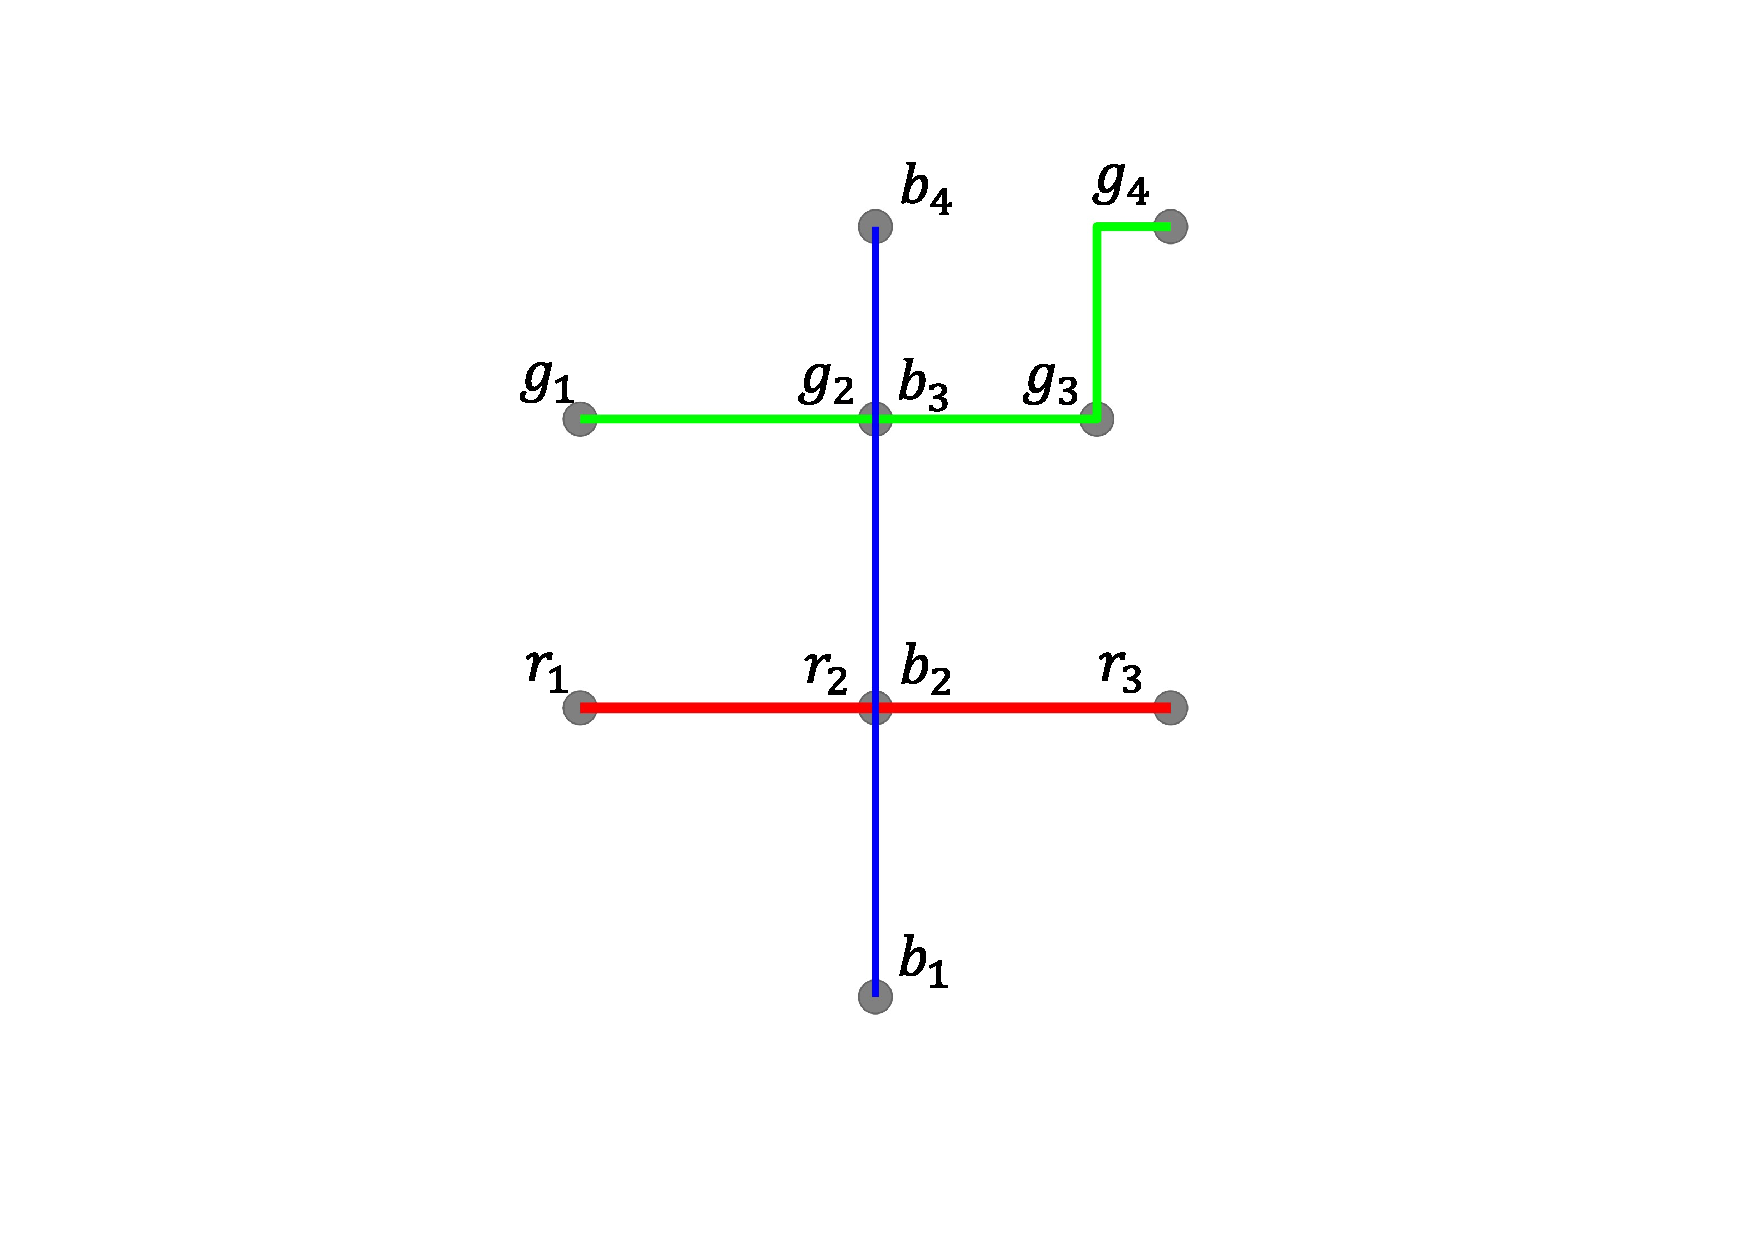
\includegraphics[width=0.34\textwidth]{figures/cross1.pdf}
%    }
%	\subfloat[\scriptsize After first swap]{
%				  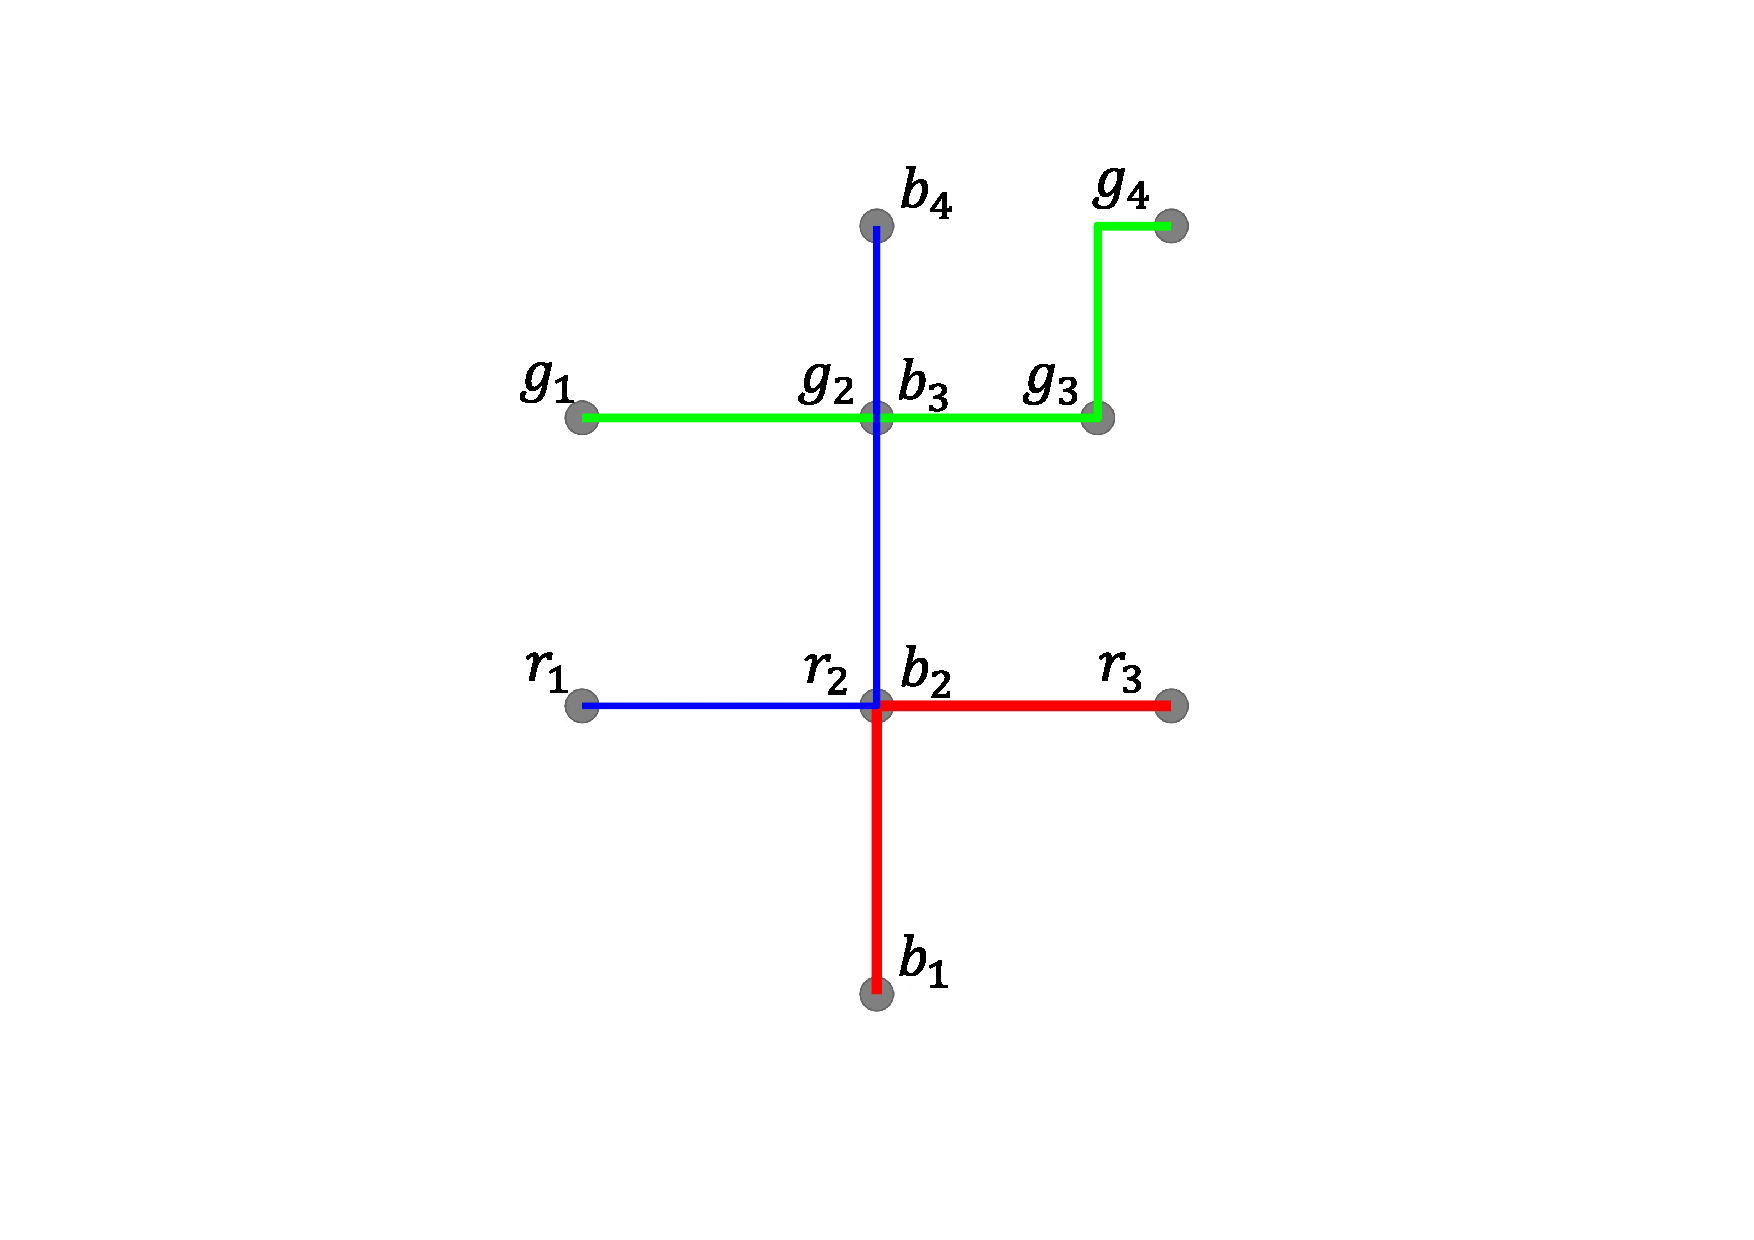
\includegraphics[width=0.34\textwidth]{figures/cross2.pdf}
%   	}
%    \subfloat[\scriptsize After second swap] {
%				  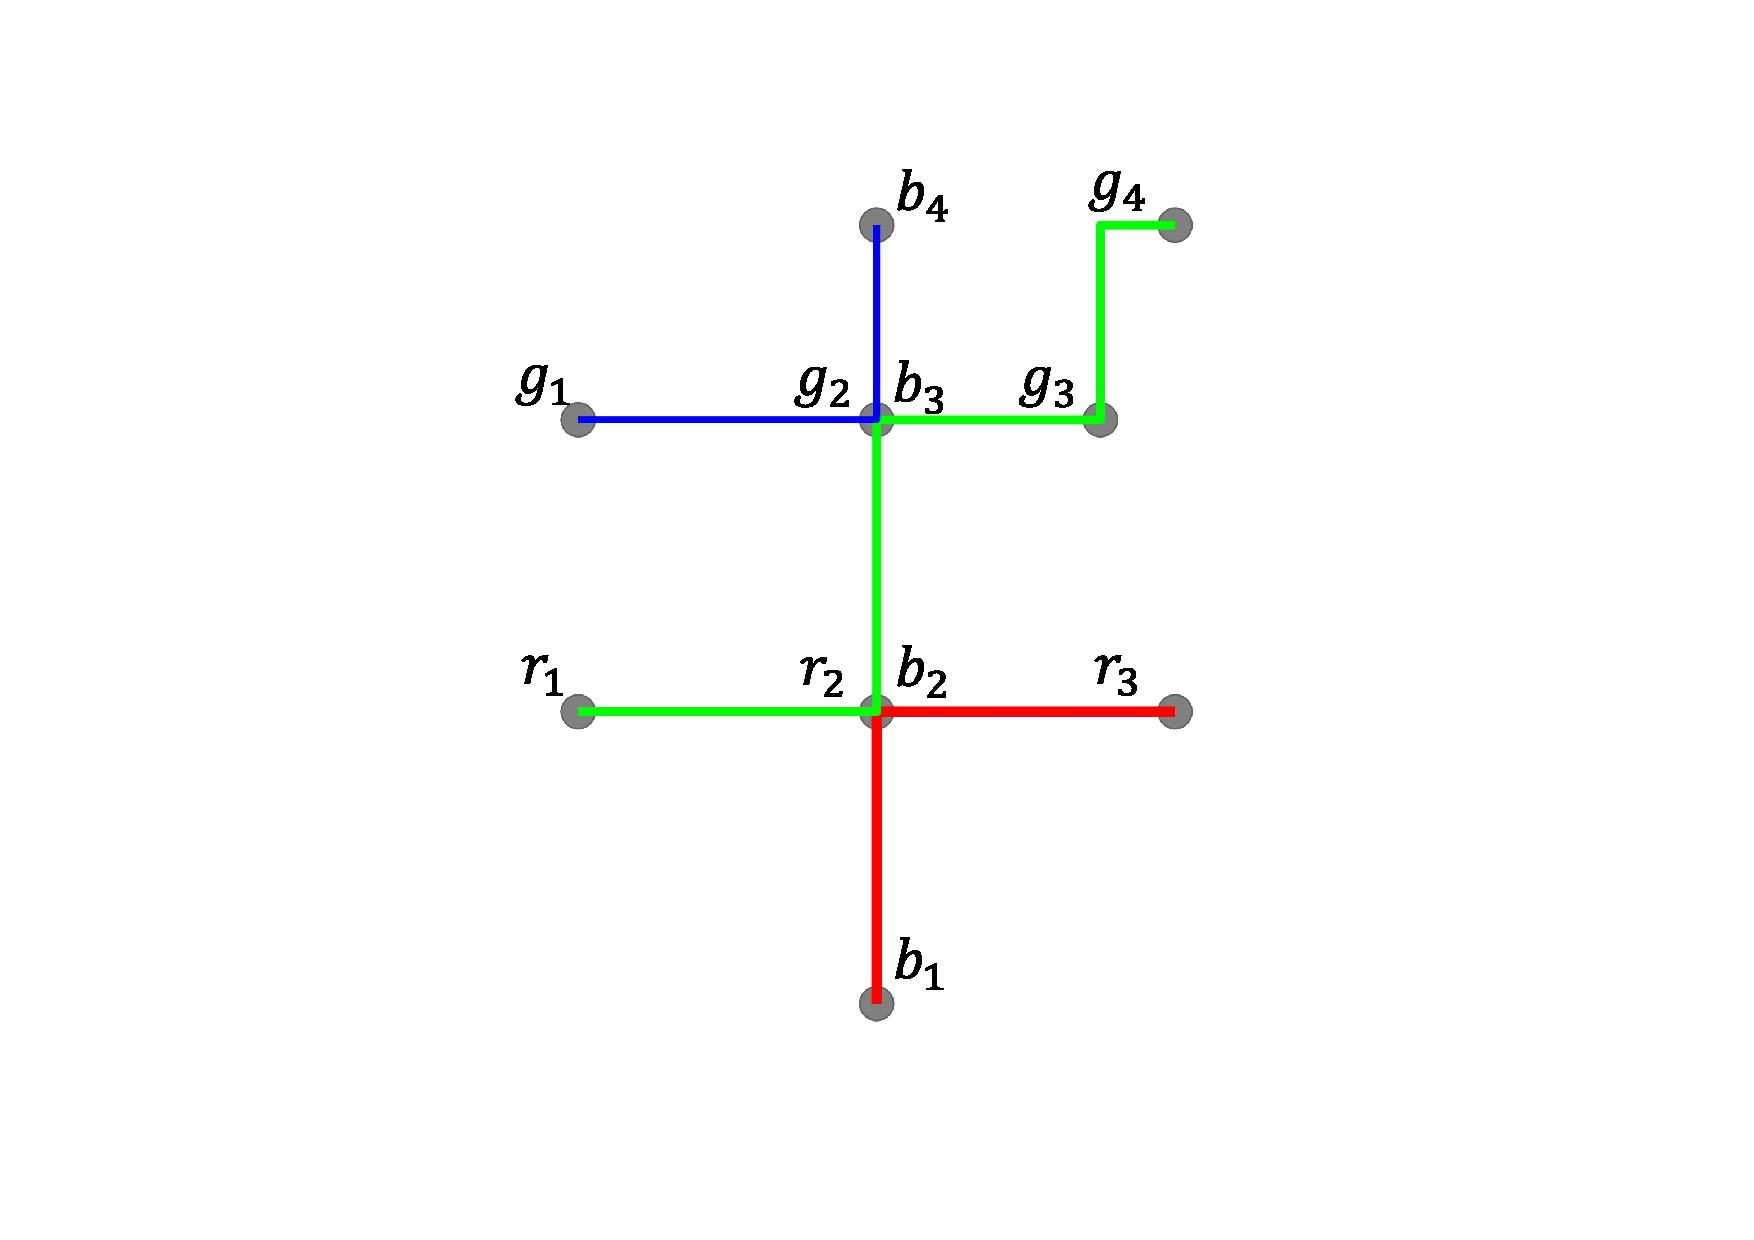
\includegraphics[width=0.34\textwidth]{figures/cross3.pdf}
%   	}
%\caption{Three trajectories before and after swapping}
%\label{fig:swap}
%}
%\end{figure*}
%
%
%In Figure \ref{fig:swap}, we present an example of three simple trajectories crossing $T_r, T_g, T_b$. We assume that they are moving from left to right and upwards, $T_r = (r_1, r_2, r_3)$, $T_g = (g_1, g_2, g_3, g_4)$ and $T_b = (b_1, b_2, b_3, b_4)$. Note that we are also assuming that the blue trajectory meets the red trajectory first ($b_2 \approx r_2$) and then the green trajectory ($b_3 \approx g_2$). In this tiny example, we can see how the iterative swaps preserve parts of the trajectory intact, but at the end each trajectory has parts of many others, such as the green one which ends having a segment of the blue trajectory, a segment of the red and a segment of its original trajectory $Sw(T_g)=(r_1, r_2, b_3, g_3, g_4)$.
%
%
%\begin{algorithm}[t]
%\SetAlgoNoLine
%\KwIn{Trajectory Database. Thresholds for time $\tau$ and proximity $\chi$. }
%\KwOut{Swapped trajectories identifiers $Sw(T_i)$.}
%
%Partition the timestamps $t =\bigcup \tau_j$ in intervals of length $\tau$
%
%\For{each pair of registers $i,j$ in interval $\tau_j$}{
%  \If{ $dist(l_i, l_j)< \chi$}{
%    add $i,j$ to close records list (possible swaps) $S_{\tau_j}$ at the given time interval.
%  }
%}
%generate random matching with possible swaps in $S_{\tau_j}$\
%
%order all swaps in $\bigcup S_{\tau_j}$ by timestamp\
%
%\For{each pair $i\approx j$ in $\bigcup S_{\tau_j}$}
%{swap $T_i$ with $T_j$}
%\KwRet {Swapped trajectories $Sw(T_i)$}
%
%\caption{Offline algorithm for swapping trajectories}
%\label{alg:one}
%\end{algorithm}
%

%\subsection{SwapMob sanitizer}
%****** He comentat tota aquesta seccio per nomes citar l'altre paper ******
%aqui EM FALTA explicar la definicio del SwapMob 

%
%We follow an architecture similar to \cite{Hoh06} in which a Trusted Third Party ($TTP$) knows the
%vehicles' identities but cannot access sensor information (such as position and  speed); and a Service Provider ($SP$) knows the sensor measures but not the identities.
%Further, the $SP$ calculates which records are close to each other without knowing to which individual they belong and communicates them to the $TTP$ (in this case SwapMob sanitizer) such that it can swap their identities without knowing at which location they were.

%
%This is achieved in the following way (See Figure \ref{fig:protocol}):
%\begin{enumerate}
%\item Users communicate with SwapMob, sending their sensor data ($M$) encrypted with the public key ($K_{SP}$) of $SP$. SwapMob keeps the number of register ($i$), which user has sent it ($u_i$), its current pseudonym ($ID_i$), the timestamp ($t_i$) and the encrypted sensor data $E(M_i, K_{SP})$, which includes their encrypted location ($l_i$).
%
%\item SwapMob sends the vector ($i, t_i, E(M_i, K_{SP}))$ to the $SP$, who decrypts $E(M_i, K_{SP})$ and keeps a buffer of data on interval $\tau_j$ that contains all timestamps between timestamp $t_j$ and $t_{j+1}$ and has length $\tau$, that is $\tau_j =\{ t : t_j < t < t_{j+1}\}$.
%
%\item $SP$ sends the set $S_{\tau_j}$ of registers that were at distance less than the predefined threshold $\chi$ during the interval of time $\tau_j$ back to SwapMob, more formally $S_{\tau_j} = \{ i,i' : d(l_i, l_{i'}) < \chi \mbox{ and } t_i,t_{i'} \in \tau_j\}$. SwapMob calculates the swaps and stores the users and swapped $IDs$ list,
%that is, for every record $i$ SwapMob keeps the corresponding swapped id $Sw(ID_i)$ and the user ($u_i$) to which such pseudonym corresponds.
%
%\item Finally, every given period of time which could  be daily, weekly or monthly, SwapMob reports the list  of ($i, Sw(ID_i)$) to $SP$.
%%In our example, it is reported each 24 hours at 18:05.
%
%\end{enumerate}
%The authentication data integrity of the communications can be guaranteed with a hash-based message authentication code.
%
%
%\begin{figure*}
%\center{
%  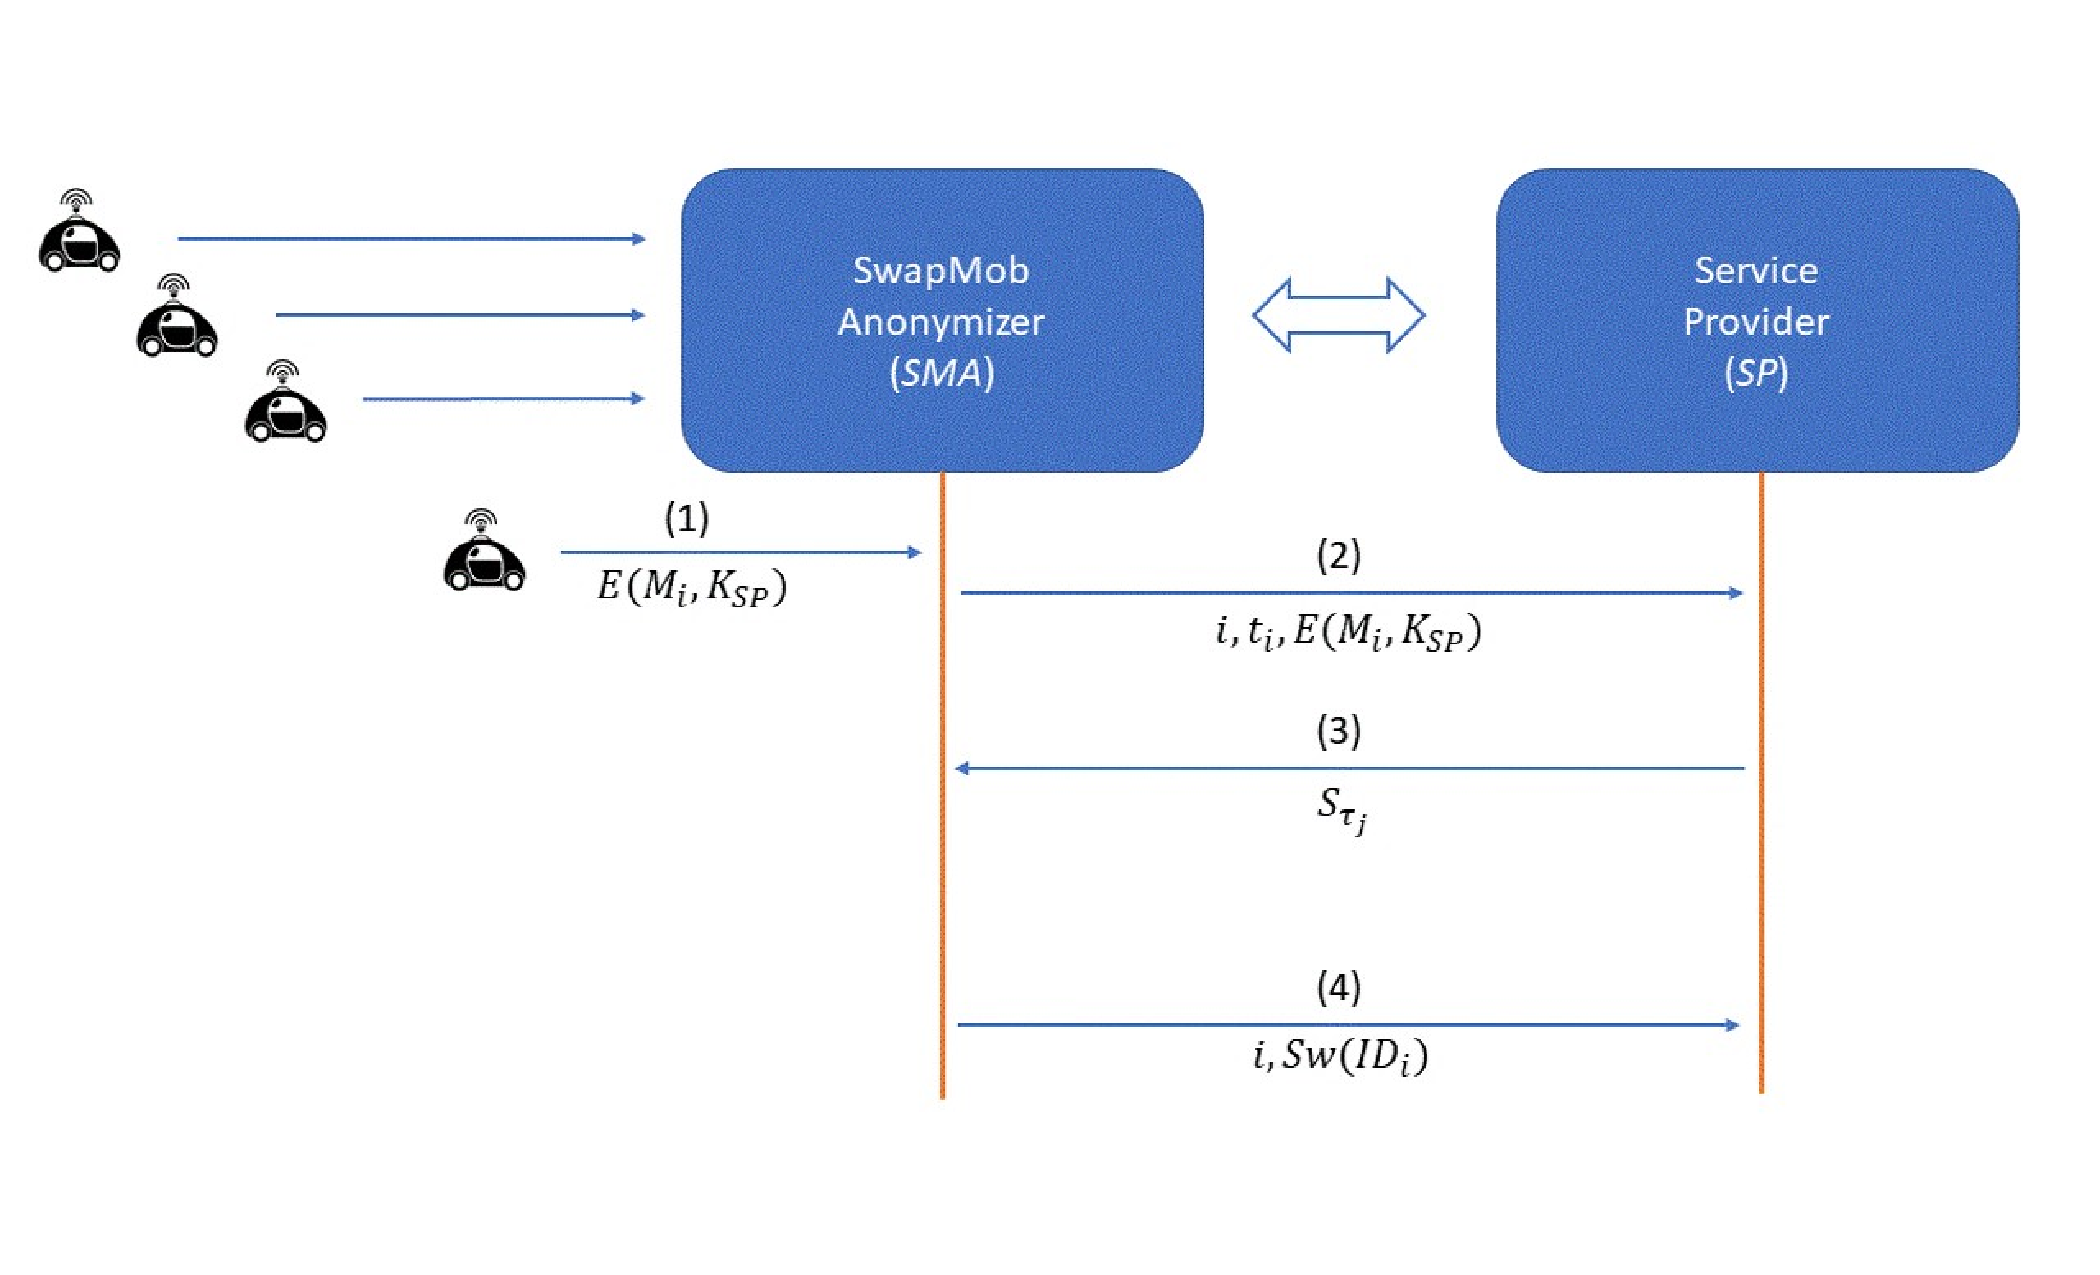
\includegraphics[width=0.95\textwidth]{figures/Protocol6.pdf}
%  \caption{Architecture of our system}
%  \label{fig:protocol}
%}
%\end{figure*}
%
%In this way, $SP$ obtains the measures of all sensors $M$ in real-time (Step 2), and at the end of the day also gets the sanitized trajectories of the users that generated them (Step 4).
%Even, though $SP$ knows which records belong to $S_{\tau_j}$ (Step 3), $SP$ does not know to which other record they have been swapped during period $\tau_j$, and by the iterative swaps it gets even harder to associate them to a specific user.
%
%At the same time, SwapMob only knows the users, the timestamps at which they have crossed, and the reported trajectories are already sanitized by SwapMob (Step 4).

%Our system, can be applied for the use case proposed in \cite{Beresford2003}, by defining a set of swap zones (similar to the mix zones) and adding the restriction that the swapping cannot be performed outside such places. Then, the spatio-temporal trajectories of users between such swap zones could be monitored in an anonymous and precise way.
%
%
%However, there will still be some differences. Namely, the swap zone that we consider is the entire application zone, whereas in \cite{Beresford2003} a user entering a mix zone can be distinguished from another user emerging from the same zone if the size of the mix zone is too large.  
%This same argument justifies that the distance and time parameters, $\chi$ and $\tau$ must not be too large either in our algorithm, otherwise swapping could not be credible.
%


%\subsection{CHECK: Protecting against reidentification} % by Home/Work location

%It is well known that de-identification does not necessarily means anonymization. The same attributes that are used for extracting knowledge, may be used for pointing to a specific individual, and uniquely relating their data to their real identity.
%
%Other notions of privacy are defined depending on the context, which may be of statistical databases \citep{Danezis15}, networks \citep{Zhou:2008}, or geo-located data.
%
%By identifying the POIs of an individual, it is possible to infer their habits (e.g., does sport, travels a lot), the locations that he visits frequently (may be related to political or religious beliefs) or even related to health (clinics, hospitals). This may also be used to infer their schedule, predict their future locations, learn their past locations and possibly even infer their personal relations by observing frequent or periodic co-locations.
%Moreover, such habits and locations can be easily used to reidentify the individuals behind the data, as it has been shown on previous studies on anonymity of home/work location.
%
%Regarding this topic, \cite{Golle:2009} showed that the sizes of the anonymity set were 1, 21 or 34980 for workers who revealed their home and work location with noise or rounding on the order of a city block, a kilometer or tens of kilometers (census block, census tract, or county), respectively. 
%That is, when the data granularity was on the order of a census block, the individuals were uniquely identifiable, and for granularities on the order of census track or county, they were protected within sets of size 21 or 34,980.
%\cite{Zang:2011} inferred the top $N$ locations of a user from call records and correlated such information with publicly-available side  information such as census data.  Then, they showed that the top 2 locations likely correspond to home and work location and that the anonymity sets are drastically reduced if an attacker infers them.
%
%Therefore, for protecting the individuals against reidentification, it is crucial to protect their home addresses and POIs, to provide them with minimum guarantees of keeping them anonymous.
%Swapped data may not allow for following a specific individual and his whereabouts, and thus, this will not permit personalization or individual classification, which are ways of protecting their privacy.
%
%A different approach regarding the possibility of reidentification and the (im)possibility of protection, is in \cite{demontjoye2013}, where they measure the uniqueness of human mobility traces depending on their resolution and the available outside information, assuming that an adversary knows $p$ random spatio-temporal points. Then, they coarsen such data spatially and temporally to find a formula for uniqueness depending on such parameters.  
%We argue that SwapMob preserves privacy by dissociating the segments of trajectories from the subject that generated them.
%
%
\subsection{Utility of swapped data as privacy-preserving decisions}\label{sect:util}
In this section and the entire paper, we are assuming that the data sanitized by SwapMob will be used for making mobility maps and predictions that may be useful for intelligent transportation systems and for planning in a city.
%
%Our main contribution here is to formalize the relationship between statistical decision procedures that are used to extract utility from the data on one hand and sanitizers that attempt to guarantee a particular measure of privacy via sanitization on the other.  

\subsubsection{Current examples:}
As \cite{Hoh2005} proposed, pre-specified vehicles could periodically send their locations, speeds, road temperatures, windshield wiper status and other information to the traffic monitoring facility. These statistics can provide information on the traffic jams, average travel time or the quality of specific roads, and can be used for traffic light scheduling and road design.

%Furthermore, the sensors do not necessarily have to be attached to vehicles, they could be carried on mobile phones, and the utility of using the individuals for sensing is preserved, since all their sensor data, including all their movements and timestamps (in aggregate) are kept intact by SwapMob.
%

In \cite{Calabrese2011}, a real-time urban monitoring platform and its application to the City of Rome was presented; they used
a wireless sensor network to acquire real-time traffic noise from different spots, GPS traces of locations from 43 taxis and 7,268 buses, and voice and data traffic served by each of the base transceiver stations from a telecom company in the urban area of Rome. These are few examples of sensors that could be carried by individuals, sanitized and transmitted to a service provider via SwapMob.

The offline mining from \cite{Yuan2011} representing the knowledge from taxi-drivers as a landmark graph may still be carried out after data anonymization with SwapMob. 
A landmark is defined as a road segment that has been frequently traversed by taxis, and a directed edge connecting two landmarks represents the frequent transition of taxis between the two landmarks. This graph is then used for traffic predictions and for providing a personalized routing service.

\subsubsection{SwapMob is a Sufficient Sanitizer:}

In general, lossless maps of flows, up to a statistical experiment and its sufficient statistics, encoded by {\em sufficiently sanitized trajectories} can be obtained by using SwapMob at several aggregation levels and time resolutions specified by $\chi$ and $\tau$, respectively.  
Next, we show that unlike $k$-anonymity and $\epsilon$-differential privacy based approaches, SwapMob does indeed preserve the sufficient statistics of counts, transition counts and ODM: the three sufficient statistics with their corresponding statistical experiments described in Section~\ref{Sec:SufficientSanitizer}.

It is easy to see that the SwapMob sanitizer for a given time interval $\tau$ and spatial resolution specified by $\chi$, preserves the sufficient statistics of counts in each cell or state given by the $\tau,\chi$-specified spatial partition.  
First, the swapping operation within each cell only swaps random pairs of trajectories within it and thus leaves the counts invariant.  
Also, the points of entry and exit for each trajectory for a given spatio-temporal cell are preserved as the swapping operation only happens across random pairs of trajectories inside the cell.  
Thus, the number of transitions between any two spatio-temporal cells will also be preserved.  
This actually preserves the sufficient statistics for the time-inhomogeneous Markov chain and not merely that of the time-homogeneous Markov chain. 
Note that, although we have discussed about discrete time Markov chains specified by units of $\tau$, we can just as easily generalize the underlying models to continuous-time Markov chains by appropriate projections and the use of timestamp information in the trajectories.   


%\subsection{Privacy measure: Adversary Information Gain}\label{Sec:InfoGain}
%*** Measure from: "Sanitizing and measuring privacy of large sparse datasets for recommender systems".
%
%The level of privacy provided by an algorithm is commonly measured with the a priori guarantees of $k$-anonymity or $\epsilon$-differential privacy, in which tuning the parameters of $k$ and $\epsilon$ increases or decreases the level of privacy.
%Also, the concept of unicity from \cite{demontjoye2013} may be related to privacy of mobility data, because an adversary having auxiliar (external) information may uniquely identify an individual in the database by relating such information with a unique record.
%
%
%Our assumption here, is that the adversary knows a precise point (location and timestamp) that uniquely identifies an individual. This means that the adversary can link such point to the sanitized individuals' data. 
%
%This is in contrast to the three methods for measuring privacy that we have just mentioned.
%Firstly, in $k$-anonymity there are not unique Quasi-Identifiers and their combinations are repeated at least $k$-times. Secondly, for $\epsilon$-differential privacy, the presence of an individual in the database is not revealed (up to $\epsilon$). Finally, in  the unicity tests from \cite{demontjoye2013} the location and timestamp data is published up to some resolution. 
%
%
%Therefore, we define the \emph{Adversary Information Gain (AIG)}, as the fraction of the original trajectory that is disclosed by an adversary who knows a point of it. Or equivalently, the amount of additional information that an adversary can gain after linking a known point to a trajectory in the sanitized database.
%Here, we consider Adversary Information Gain in terms of the number of measurements, but elapsed time and distance traveled would both be other natural choices.
%
%We consider that an adversary can propagate his knowledge of one data point to the whole segment in-between swaps: we assume that the adversary follows the trajectory from the known measurement forward in time until the next swap occurs and also backwards in time until the previous swap has occurred. 
%The adversary will know with certainty that such segment belongs to the same individual, since no swaps were performed on it, but after the swaps will not know which path belongs to the original trajectory.
%We will show, in Section \ref{sec:reidentification}
%that in most cases, only a small fraction of the full trajectory is disclosed.


\section{Empirical evaluation}\label{Sec:evaluation}
We tested our algorithm on the T-drive dataset
\citep{Yuan2010,Yuan2011} which contains the GPS trajectories of
10,357 taxis during the period of Feb. 2 to Feb. 8, 2008 within
Beijing. The total number of points in this dataset is about 15
million and the total distance of the trajectories reaches nearly 9
million kilometers. It is important to note that not all taxis appear
every day and not all report their positions at the same interval. The
average sampling interval is about 177 seconds and 623 meters. Each
measurement contains the following data: taxi ID, date time,
longitude, latitude.

\subsection{Applying SwapMob on the data}
Before applying SwapMob to the dataset, we perform some cleaning of the
data. We begin by removing all measurements for which the latitude and
longitude is outside the box $[115, 117] \times [39, 41]$, these
measurements are far outside Beijing and most of them have both
latitude and longitude equal to zero, which indicates that the
measurement is most likely not valid. W%e then remove all trajectories
%which have no measurements belonging to them at all. 
%This removes 756,561 invalid measurements and 77 trajectories that have no
%measurements in this area, and w
e end up with 10280 trajectories and 16,906,423
measurements.

For applying SwapMob we consider two taxis co-located if they are in
the same spatio-temporal cell: the spatial cell is given by a square of side-length 0.001 degrees ($\chi = 0.001$), about 111
meters, and the temporal interval is specified by being in the same minute ($\tau = 60$). 
Note that this is about 6 and 3 times less than the average sampling interval for distance and time, respectively, in the dataset.

With these parameteres, the number of possible swaps between all the
trajectories is 641,262. The average number of swaps for each
trajectory is 137. Of all the 10,280 trajectories there are only 772 trajectories with less than 20 swaps, and their distribution is depicted in Figure
\ref{fig:swaps-distribution}. There are 324 trajectories that do not
participate in any swaps at all, however 265 of these trajectories
have less than 10 measurements (compared to an average of more than
1000). 

\begin{figure}
%  \subfloat[\scriptsize Frequency histogram of number of swaps for all
%  the 772 trajectories participating in less than 20 swaps.] {
    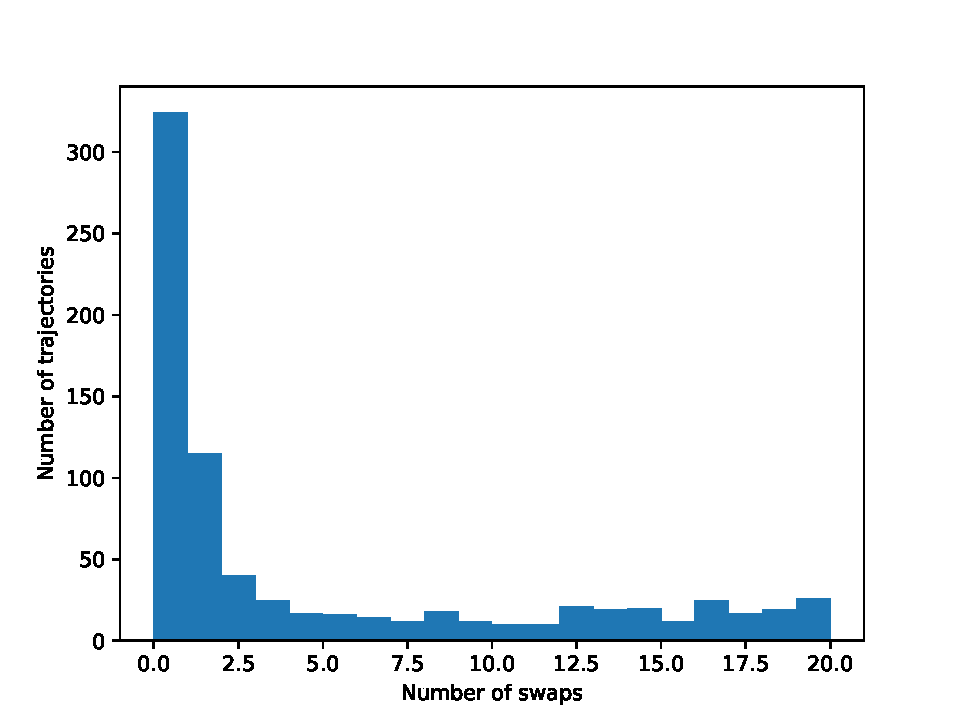
\includegraphics[width=0.45\textwidth]{figures/swaps-distribution-20.pdf}
%    \label{fig:swaps-distribution-20}
%  }
%  \hfil
%  \subfloat[\scriptsize Frequency histogram of number of swaps for all
%  trajectories.] {
%    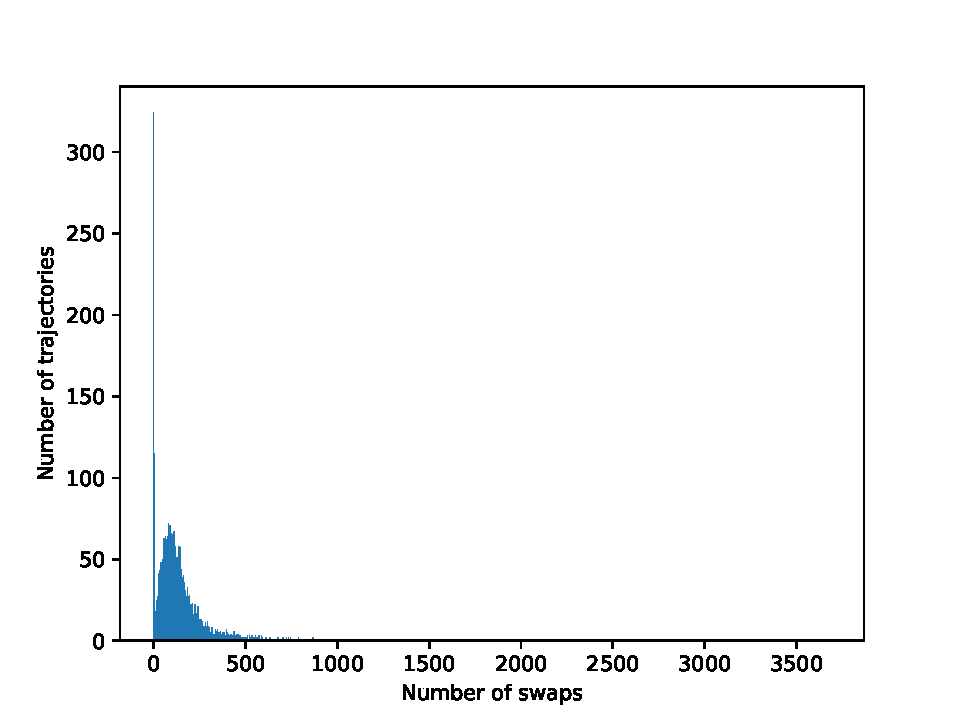
\includegraphics[width=0.5\textwidth]{figures/swaps-distribution-all.pdf}
%    \label{fig:swaps-distribution-all}
%  }
  \caption{Frequency histograms of number of swaps for trajectories participating in less than 20 swaps.}
  \label{fig:swaps-distribution}%
\end{figure}

%\subsection{Adversary Information Gain}
\subsection{Privacy measure: Adversary Information Gain}\label{Sec:InfoGain}
 
For measuring privacy we will define the Adversary Information Gain measure adapting the Sensitive Attribute Risk measure from \cite{Salas:2019}. Sensitive Attribute Risk considers the fraction of the published attributes of an individual that is part of its original attributes. 

By considering the sensitive attributes to be locations instead of movies in recommender systems, the Adversary Information Gain (AIG) here is the fraction of the original trajectory that is disclosed by an adversary who knows a point of it.
We consider that an adversary can propagate his knowledge of one data point to the whole segment in-between swaps: we assume that the adversary follows the trajectory from the measurement forward and backward in time until the next and previous swaps occured. 
%Then, we have to measure the 
%length of the segments between the swaps. 
%Since every trajectory
%participates in an average of 137 swaps and is thus split into an
%average of 138 segments. Knowing one point the adversary will learn
%one of these segments. 
For each trajectory, we can look at the longest such segment and compare its length to that of the
whole trajectory. 
We plotted the distribution function of such measure in Figure \ref{fig:ECDF-max-part-OD} with grid size = None. It shows that, for more than 75\% of all
trajectories, the AIG is less than 0.2, for 90\% of the trajectories it is less
than 0.4. For most trajectories, an adversary will thus learn only a
small fraction of the original trajectory.

%We can also consider the case when the adversary knows several points
%of the trajectory. If the extra points lie on the same segment of the
%trajectory as the first one, no more knowledge is gained. However, if
%the extra points lie on other segments of the trajectory, the adversary
%learns also these and more of the trajectory is disclosed. If the
%adversary knows several segments of the trajectory, it can also try to
%infer which way was taken between them, and thus learning more than
%just the disclosed segments. Analysing this is however outside the
%scope of this article and left as further research.


%\begin{figure}[h]
%  \center
%  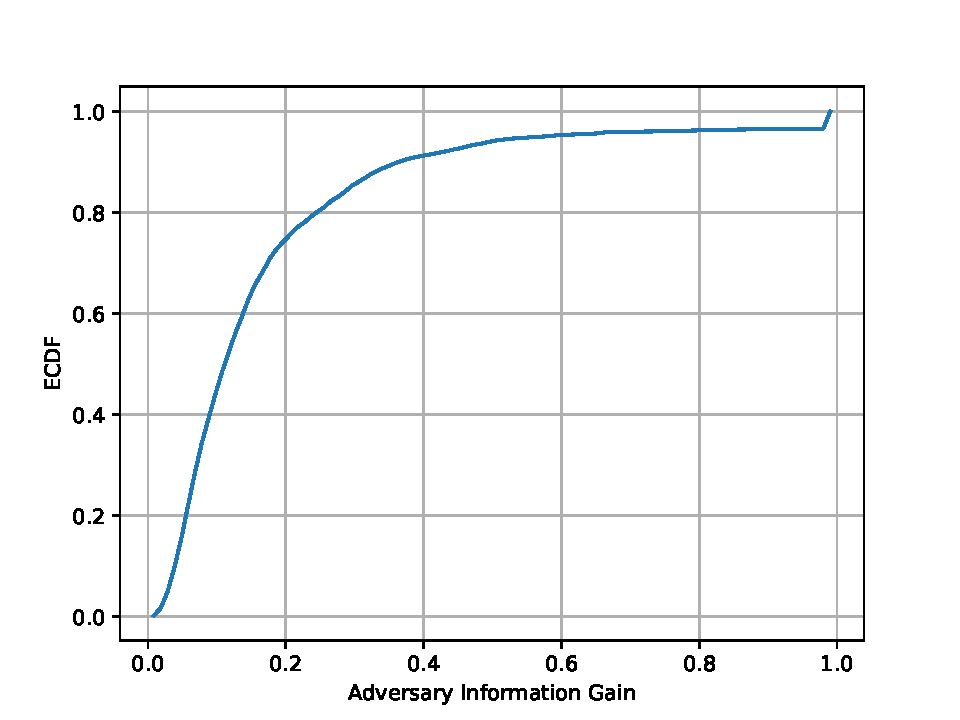
\includegraphics[width=0.45\textwidth]{figures/ECDF-max-part.pdf}
%  \caption{Cummulative Distribution Function of Adversary Information Gain.}
%  \label{fig:ECDF-max-part}
%\end{figure}

\subsection{Privacy when preserving the Origin-Destination Matrix}\label{S:PrivacyODM}
We now consider the effects on the privacy measures of restricting 
swapping to preserve the Origin-Destination Matrix (ODM), introduced in Section~\ref{Sec:SufficientSanitizer}. That is, for two trajectories to
swap they have to share the same starting location or origin and ending location or destination (up to some scale).  
This is in addition to the earlier requirements for allowing a swap ($\tau$, $\chi$).

We define the states or locations used in the ODM by the labelled cells or states in a grid obtained by partitioning the
city into equally sized squares (in units of degrees).  
%Bigger squares give a coarser grid and smaller squares a finer grid.  
%
%The resolution of the grid is given by the width or side-length of the squares in degrees of latitude and
%longitude (1 degree of latitude is about 111,000 m in Beijing), a lower width then corresponds to a finer grid. 
The start location or origin for a trajectory will be given by the square that its first
measurement belongs to and the end location or destination by the square that its last
measurement belongs to. 
In general, it might be more appropriate to
have start and end locations to be determined by the location of the
trajectory at a certain time of the day. 
However, for keeping it
simple, we choose to use only the first and last measurement.
More generally, our approach allows for an arbitrary set of subsets of the city and arbitrary time-intervals to specify Origins and Destinations in a single ODM, or even a sequence of ODMs, but we use a simple grid-based partition at different spatial resolutions to illustrate the effects on privacy here.  

We analyze how the preserved privacy changes when we go from having
no grid to having a very coarse grid and then making it finer and
finer.

\begin{figure*}
\centering
  \subfloat[\scriptsize The number of possible swaps depending on the
  grid size. Going from having no grid to a very fine grid.] {
    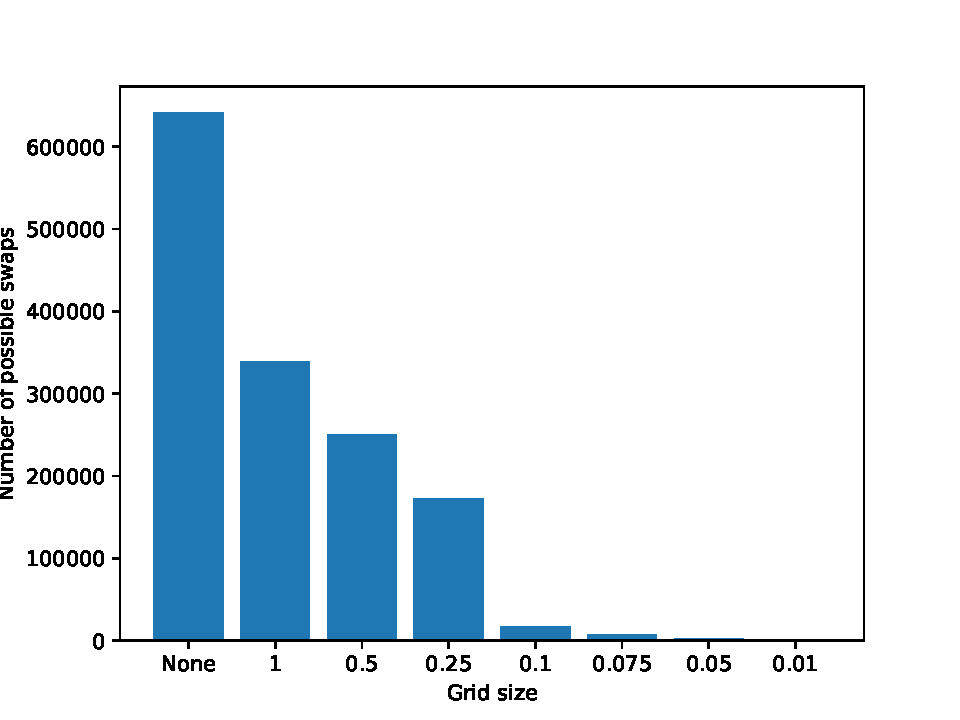
\includegraphics[width=0.45\textwidth]{figures/num-swaps-OD.pdf}
    \label{fig:num-swaps-OD}
  }
%  \hfil
  \subfloat[\scriptsize Empirical Cummulative Distribution Functions of the Adversary Information Gain for different grid
  sizes.] {
    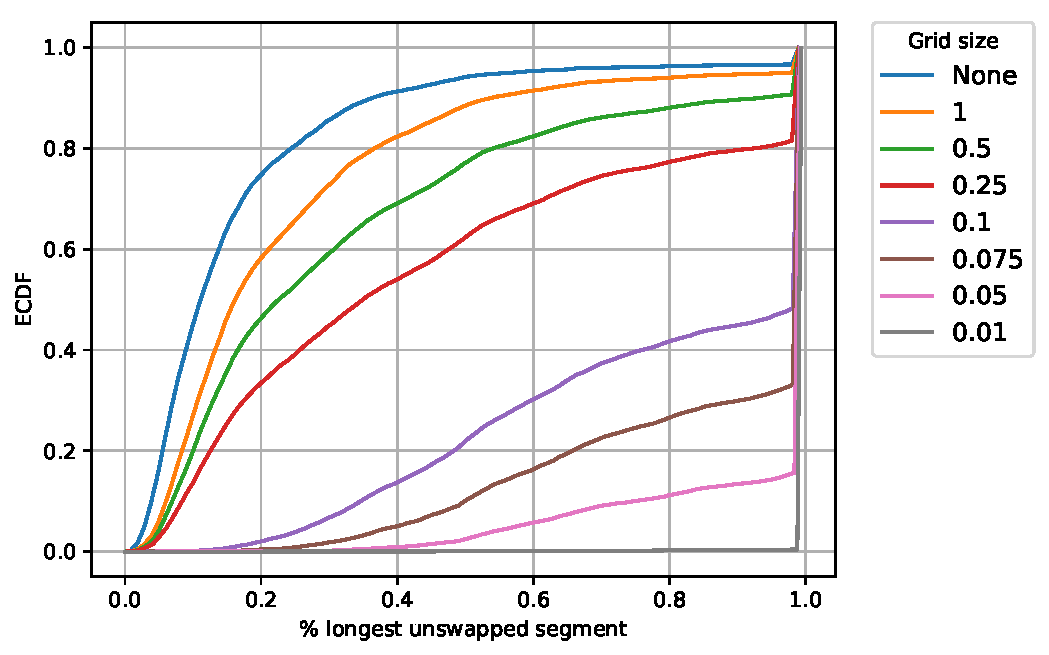
\includegraphics[width=0.45\textwidth]{figures/ECDF-max-part-OD.pdf}
    \label{fig:ECDF-max-part-OD}
  }
  \caption{Preserved privacy when also preserving the ODM}
  \label{fig:OD}
\end{figure*}

In Figure \ref{fig:num-swaps-OD} we see how the number of possible
swaps change when we make the grid finer. At first, we have the number
of swaps without a grid and then we have the numbers for grids of
squares of the given height. The largest height used is 1 degree
%, which can be compared to the distance of 0.001 degrees, that we used for determining if two trajectories are swappable, i.e.~close enough to be swapped.  
This grid splits the city into four parts, of which two contain
most of the measurements. On the other extreme, the finest grid is made up of squares of width 0.01 degrees which is 10 times the proximity threshold for swappability.  
We see that the number of possible swaps quickly decreases as the grid
gets finer. 
%Even at the coarsest grid, the number of swaps is halved
%compared to having no grid. When the grid height goes below 0.1 we have
%very few possible swaps.

Since the preserved privacy heavily depends on the number of possible
swaps, we expect it to quickly decrease as the grid becomes finer, see Figure
\ref{fig:ECDF-max-part-OD}. 
%The line corresponding to having no grid
%is the same as in Figure \ref{fig:ECDF-max-part} and we can see that
%the privacy decreases as the grid becomes finer.

We can conclude that the preserved privacy is greatly influenced by
the grid size of the ODM. If the grid is too fine almost no swaps occur
and the SwapMob algorithm is not efficient. For very coarse grids the
privacy is still reduced but depending on the application it could still
be considered acceptable.  
Furthermore, by defining a sequence of ODMs, say $(M_1,M_2,\ldots,M_m)$, specified by arbitrary subsets of space 
and intervals of time $[t_{i,o},t'_{i,o}]$ and $[t_{i,d},t'_{i,d}]$ for each $M_i$, one can increase privacy by increasing the number of swappable trajectories. Such a sequence of ODMs should generally be of greater utility for certain decision problems. We defer a thorough investigation of sufficient sanitizers that preserve sufficient statistics for such sequences of ODMs across spatial and temporal resolutions in a principled manner for future research.  

\section{Conclusions}\label{Sec:conclusions}

%We have defined and tested a novel algorithm for mobility data 
%sanitization that consists of swapping trajectory segments. In contrast to the $k$-anonymity or differential privacy models for trajectory sanitization, the proposed method does not modify the data, but its association to specific individuals, and it is performed in real time, without the need of having the entire dataset.
%
%The proposed protocol tackles both identity and location privacy,
%and our data model can be adapted to protect either single trajectory positions, as they lose the relation to the individual who has generated the data, or the whole trajectories, since they are mixed among many different peers.

We have defined the concept of sufficient sanitizer in an approach to utility first data protection methods in which the utility requirement (as an statistic) is a priori defined, then the sanitization algorithm that preserves such utility is applied to the data.

We showed that the SwapMob algorithm is a sufficient sanitizer. When applied in real time it may be useful for providing anonymous data to personalized assistants. 

We tested the SwapMob algorithm on the T-drive dataset to show that a high number of swaps occur and
most trajectories participate in several swaps. The
original trajectories are split up into many smaller segments, hence SwapMob prevents an adversary who may know exact points of the trajectory from inferring much of the full trajectory, this is measured with the Adversary Information Gain.

%This is expressed as the Adversary Information Gain, 
%which we formally defined to measure the capability of an adversary to leverage his knowledge of a given exact point, to infer a larger segment of the sanitized trajectory.

However, when adding
the utility restriction of preserving the ODM, the number of swaps quickly
decreases and it becomes much easier for an
adversary to infer a bigger portions of the trajectories in the database.

This is the natural tradeoff between the {\em societal utility} gained through the preservation of the ODM, where ODM is a sufficient statistic, and the {\em individual privacy lost} by the sufficient sanitizer.

%We have simulated our protocol with an offline algorithm. Although, the protocol could be run in real time in which data is transmitted by user devices to our sanitizer that communicates and collaborates with a server. By changing the sanitizer for a group protocol, the protocol could provide security against collusion between the service provider and the sanitizer.


%It must be mentioned that swapping cannot be carried out when an individual does not come close to anyone along their path. 
%Hence, the proposed technique will not protect an individual who does not proximally encounter anyone in their daily activity.  
%We consider that it is not very common for an individual to spend too much time without meeting someone or going out from home. Moreover, such individuals can be kept outside the database without compromising its utility, e.g., in the case of T-drive data 265 of these 324 trajectories have less than 10 measurements (compared to an average of more than 1000).


We remark that preserving sufficient statistics for various statistical decision problems is used in traffic engineering and city planning, including exact count queries, transition count queries and ODM queries, which neither $k$-anonymity nor differential privacy cannot formally guarantee.


A formal privacy-preserving decision-theoretic framework based on probabilistic models and statistical experiments for co-trajectories that can be integrated across multiple spatial and temporal resolutions needs further investigations, especially when the computational setting becomes distributed to handle mobility data at a massive scale.

\section*{Acknowledgements}
Juli\'{a}n Salas acknowledges the support of a UOC postdoctoral fellowship.
This work is partly funded by the Spanish Government through grants  RTI2018-095094-B-C22 ``CONSENT" and TIN2014-57364-C2-2-R ``SMARTGLACIS'', Swedish VR (project VR 2016-03346). Raazesh Sainudiin was partly funded by Combient Competence Centre for Data Engineering Sciences at Uppsala University and the Research Center for Cyber Security at Tel Aviv University established by the State of Israel, the Prime Minister's Office and Tel-Aviv University.
%Juli\'{a}n Salas acknowledges the support of a UOC postdoctoral fellowship.
%The above line is already the same as the first line. So it is commented out. Raaz - Fri Jul 26 18:25:49 CEST 2019



\bibliographystyle{model2-names}

\bibliography{biblio-swap2}

\end{document}

%%
